%%%%%%%%%%%%%%%%%%%%%%%%%%%%%%%%%%%%%%%%%
% Beamer Presentation
% LaTeX Template
% Version 1.0 (10/11/12)
%
% This template has been downloaded from:
% http://www.LaTeXTemplates.com
%
% License:
% CC BY-NC-SA 3.0 (http://creativecommons.org/licenses/by-nc-sa/3.0/)
%
%%%%%%%%%%%%%%%%%%%%%%%%%%%%%%%%%%%%%%%%%

%----------------------------------------------------------------------------------------
%	PACKAGES AND THEMES
%----------------------------------------------------------------------------------------

\documentclass{beamer}

\mode<presentation> {

% The Beamer class comes with a number of default slide themes
% which change the colors and layouts of slides. Below this is a list
% of all the themes, uncomment each in turn to see what they look like.

%\usetheme{default}
%\usetheme{AnnArbor}
%\usetheme{Antibes}
%\usetheme{Bergen}
%\usetheme{Berkeley}
%\usetheme{Berlin}
%\usetheme{Boadilla}
%\usetheme{CambridgeUS}
%\usetheme{Copenhagen}
%\usetheme{Darmstadt}
%\usetheme{Dresden}
%\usetheme{Frankfurt}
%\usetheme{Goettingen}
%\usetheme{Hannover}
%\usetheme{Ilmenau}
\usetheme{JuanLesPins}
%\usetheme{Luebeck}
%\usetheme{Madrid}
%\usetheme{Malmoe}
%\usetheme{Marburg}
%\usetheme{Montpellier}
%\usetheme{PaloAlto}
%\usetheme{Pittsburgh}
%\usetheme{Rochester}
%\usetheme{Singapore}
%\usetheme{Szeged}
%\usetheme{Warsaw}

% As well as themes, the Beamer class has a number of color themes
% for any slide theme. Uncomment each of these in turn to see how it
% changes the colors of your current slide theme.

%\usecolortheme{albatross}
%\usecolortheme{beaver}
%\usecolortheme{beetle}
%\usecolortheme{crane}
%\usecolortheme{dolphin}
%\usecolortheme{dove}
%\usecolortheme{fly}
%\usecolortheme{lily}
%\usecolortheme{orchid}+
%\usecolortheme{rose}
%\usecolortheme{seagull}
%\usecolortheme{seahorse}
%\usecolortheme{whale}
%\usecolortheme{wolverine}

%\setbeamertemplate{footline} % To remove the footer line in all slides uncomment this line
\setbeamertemplate{footline}[page number] % To replace the footer line in all slides with a simple slide count uncomment this line

\setbeamertemplate{navigation symbols}{} % To remove the navigation symbols from the bottom of all slides uncomment this line
}

\usepackage{listings}
\usepackage{amsmath}

\usepackage{graphicx} % Allows including images
\usepackage[font=small,labelfont=bf]{caption}
\usepackage{booktabs} % Allows the use of \toprule, \midrule and \bottomrule in tables

\usepackage[ngerman]{babel}
\usepackage[utf8]{inputenc}

%----------------------------------------------------------------------------------------
%	TITLE PAGE
%----------------------------------------------------------------------------------------

\title[Erkennung von erkrankten Nutzpflanzen]{Erkennung von erkrankten Nutzpflanzen anhand von Sentinel-2-Multispektralaufnahmen} % The short title appears at the bottom of every slide, the full title is only on the title page

\author{Simon Hüning} % Your name

\institute[] % Your institution as it will appear on the bottom of every slide, may be shorthand to save space
{
Universität Leipzig \\ % Your institution for the title page
\medskip
}
\date{11. Dezember 2018} % Date, can be changed to a custom date

\begin{document}

\begin{frame}
\titlepage % Print the title page as the first slide
\end{frame}

\begin{frame}
\frametitle{Inhalt} % Table of contents slide, comment this block out to remove it
\tableofcontents % Throughout your presentation, if you choose to use \section{} and \subsection{} commands, these will automatically be printed on this slide as an overview of your presentation
\end{frame}

%----------------------------------------------------------------------------------------
%	PRESENTATION SLIDES
%----------------------------------------------------------------------------------------

\begin{frame}\section{Wiederholung}\frametitle{Wiederholung}
\begin{minipage}{0.5\textwidth}
	\begin{itemize}
		\item Sentinel-2-Plattform zur Erdüberwachung
		\item Chlorophyllgehalt steht in Verbindung zur Gesundheit der Pflanze
		\begin{itemize}
			\item lässt sich durch Multispektralaufnahmen messen
		\end{itemize} 
	\end{itemize}
\end{minipage}
\hspace{1em}
\begin{minipage}{0.4\textwidth}
	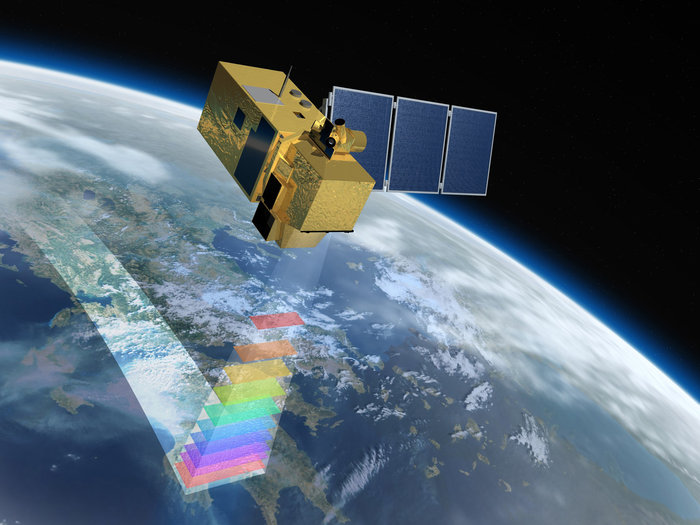
\includegraphics[width=1\linewidth]{pics/sentinel-2-scanning}
	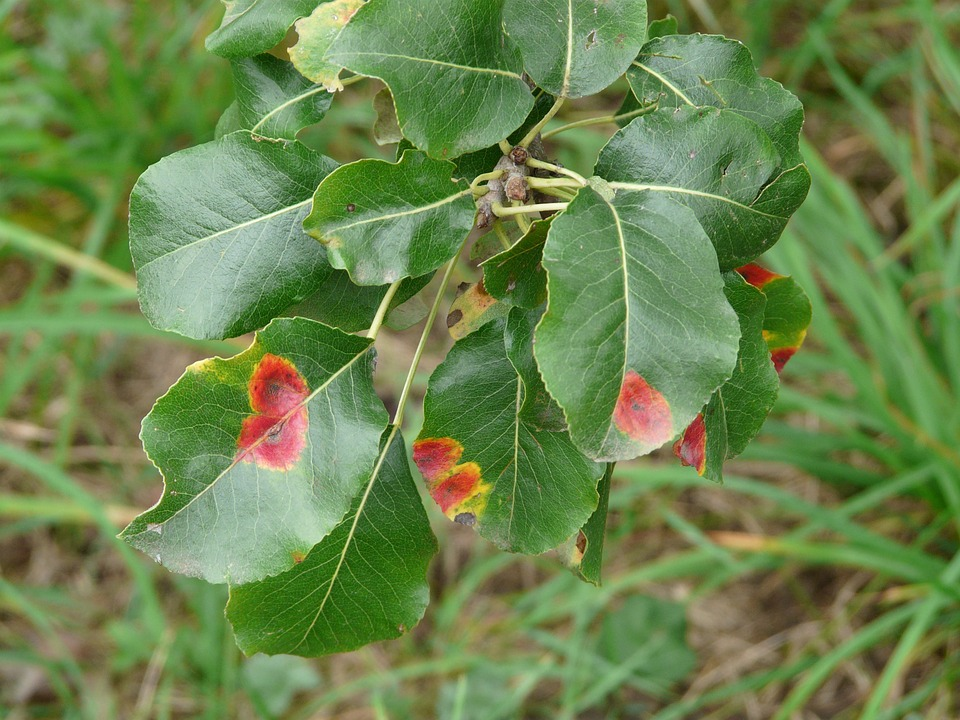
\includegraphics[width=1\linewidth]{pics/befall}
\end{minipage}
\end{frame}

%------------------------------------------------

\begin{frame}\section{Workflow}\frametitle{Workflow}
\begin{minipage}{\textwidth}
	\center
	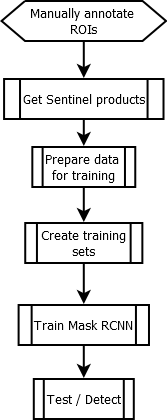
\includegraphics[width=.25\linewidth]{pics/overview}
\end{minipage}
\end{frame}

%------------------------------------------------

\begin{frame}\section{Annotierung}\frametitle{Annotierung}
\begin{minipage}{0.5\textwidth}
	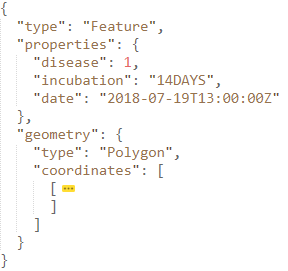
\includegraphics[width=1\linewidth]{pics/geojson}
\end{minipage}
\hspace{1em}
\begin{minipage}{0.4\textwidth}
	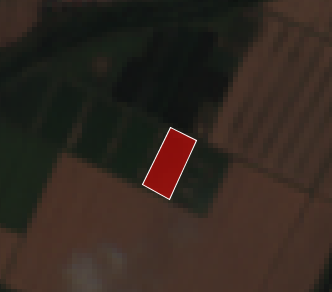
\includegraphics[width=1\linewidth]{pics/fields}
	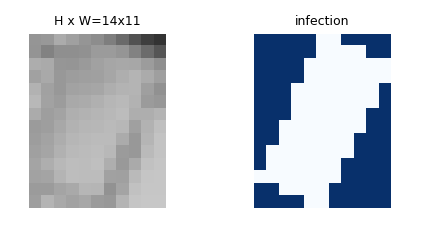
\includegraphics[width=1\linewidth]{pics/roi_mask}
\end{minipage}
\end{frame}

%------------------------------------------------

\begin{frame}\section{NDVI}\frametitle{NDVI}
	\begin{itemize}
		\item Normalized Difference Vegetation Index
		\begin{equation*}
			NDVI = \frac{Band_{NIR} - Band_{Red}} {Band_{NIR} + Band_{Red}}
		\end{equation*}
		\item wird häufig benutzt, um die Vitalität einer Pflanze zu bestimmen
		\item je mehr Chlorophyll in einer Pflanze, desto stärker die Reflexion
		\item Werte von -1 bis 1
		\item Werte $\lesssim 0$ bedeuten Wasser und je näher ein Wert an 1, desto besser gehts der Pflanze
	\end{itemize}
\end{frame}

\begin{frame}\frametitle{NDVI}
\begin{minipage}{0.4\textwidth}
	
\includegraphics[width=1\linewidth]{pics/b4}\captionof*{figure}{Red}
	
\includegraphics[width=1\linewidth]{pics/b8}\captionof*{figure}{NIR}
\end{minipage}
\hspace{2em}
\begin{minipage}{0.4\textwidth}
	
\includegraphics[width=1\linewidth]{pics/ndvi}\captionof*{figure}{NDVI}
\end{minipage}
\end{frame}

%------------------------------------------------

\begin{frame}\section{Training}\frametitle{Training}
\begin{minipage}{0.55\textwidth}
	\begin{itemize}
		\item Mask-RCNN
		\begin{itemize}
			\item Masked Region based Convolution Neural Network
			\item Entwickelt von Facebook
			\item Erweiterung von Faster-RCNN
			\item Instance Segmentation
			\item Erkennt Klassen auf Pixelebene
		\end{itemize}
		\item Training baut auf vortrainierten Gewichten auf
		\item Bewertung über mAP (mean average precision)
	\end{itemize}
\end{minipage}
\begin{minipage}{0.4\textwidth}
	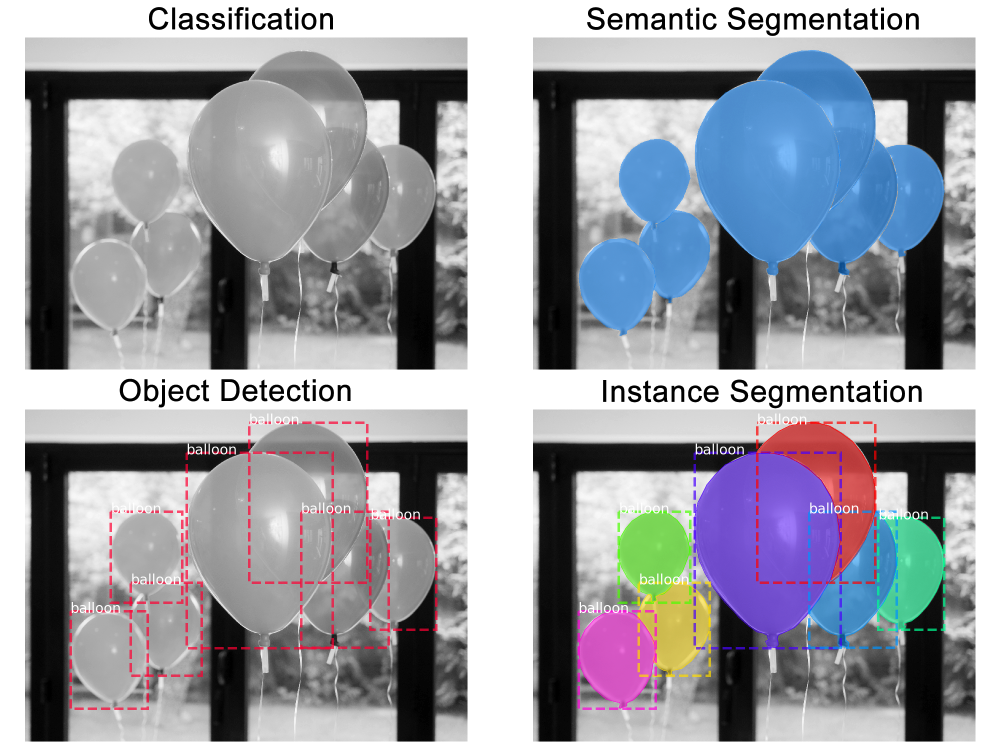
\includegraphics[width=1\linewidth]{pics/splash_balloon}
\end{minipage}
\end{frame}

\begin{frame}\frametitle{Mask-RCNN}
	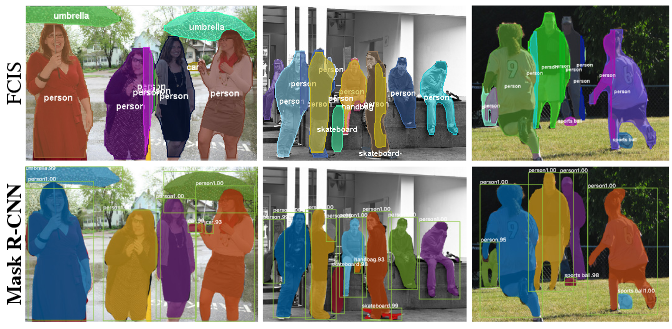
\includegraphics[width=1\linewidth]{pics/overlapping}
\end{frame}

%------------------------------------------------

\begin{frame}\section{Bisherige Versuche}\frametitle{Bisherige Versuche}
\begin{minipage}{0.5\textwidth}
	
\includegraphics[width=1\linewidth]{pics/mask}
\end{minipage}
\hspace{1em}
\begin{minipage}{0.4\textwidth}
	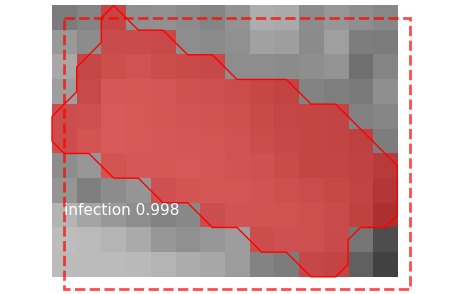
\includegraphics[width=1\linewidth]{pics/pred}
\end{minipage}
\center
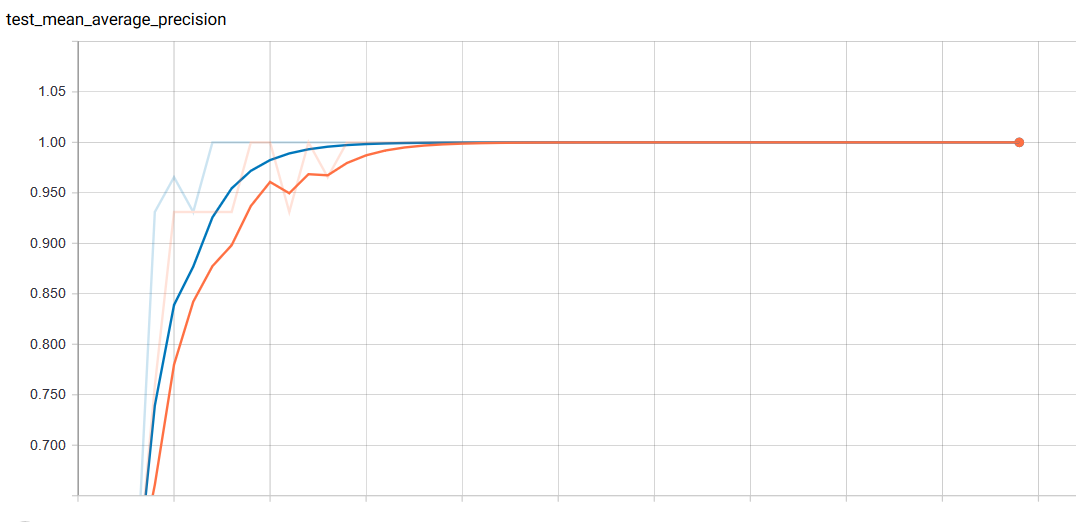
\includegraphics[width=0.7\linewidth]{pics/map}
\begin{itemize}
	\item Kleiner Datensatz -$>$ Overfitting
\end{itemize}
\end{frame}

%------------------------------------------------

\begin{frame}\frametitle{Overfitting - Was tun?}
\begin{itemize}
	\item KNN "'lernt Trainingsdatensatz auswending"'
	\begin{itemize}
		\item geringe Anwendbarkeit auf unbekannten Input
	\end{itemize}
	\item Wie lässt sich Overfitting vermeiden?
	\begin{itemize}
		\item Wenn möglich, Datensatz vergrößen
		\item Lieber simple Modelle als komplexe
		\item Augmentization
		\begin{itemize}
			\item Bild drehen, zufällige Ausschnitte, ..
		\end{itemize}
		\item Regulization
		\begin{itemize}
			\item Bevorzugt kleine Gewichte
			\item Bestraft hohe Gewichte
		\end{itemize}
		\item Training verschiedener Neuronenschichten in Intervallen
	\end{itemize}
\end{itemize}
\end{frame}

%------------------------------------------------

\begin{frame}\section{Zeitplan}\frametitle{Zeitplan}
\begin{tabular}{l l}
Dezember 2018 & Zwischenpräsentation\\
Dezember 2018 & Start Verschriftlichung\\
Februar 2019 & Abgabe\\
Februar 2019 & Abschlusspräsentation
\end{tabular}
\end{frame}

%------------------------------------------------

\begin{frame}
\centerline{Vielen Dank für Ihre Aufmerksamkeit.}
\Huge{\centerline{Fragen?}}
\end{frame}

%----------------------------------------------------------------------------------------

\end{document} 